\chapter{Related Work}\label{sec:RelatedWork}
This is not a novel idea and there are already some completed solutions and papers written about RSS fingerprint collection using multiple devices. This chapter will describe few selected solutions close to this one as a comparison.

\section{Improving Precision by Using Multiple Wearable Devices}\label{sec:IPUMWD}
This paper focuses on improving indoor localization using BLE-based fingerprinting with multiple devices \cite{IPBLEIUMWD}. Using combination of smartphone and wear should in this case prevent signal obstruction from human body and at least one of the devices should receive beacon signal. Unfortunately due to low BLE sensibility of wear devices, authors decided to supplement them with a second mobile device, in this case with Nexus 5 running Android version 4.4.

It proposes calculating medians from 800 millisecond tests where user can move only one meter from starting position at most. Average and variance is calculated for all medians with the same position, based on these values a normal distribution is used to model the potential variation of RSSI. Important thing to note is that fingerprint maps are also built based on facing direction. These maps are then tested using five main scenarios.

\begin{itemize}
	\item P1: single device held in hand where body does not obstruct its line of sight (LOS) path to all beacons.
	\item P2: one device is placed in breast pocket where LOS may be obstructed to some beacons.
	\item P3: user holds smartphone in hand and wears a smartwatch on one wrist.
	\item P4: single device is placed in the breast pocket and the other is on one wrist.
	\item P5: one device is in the breast pocket, and two other devices, each on one wrist.
\end{itemize} 

At first, four of these scenarios were tested in a 15x8 meters entrance hall with four deployed beacons in the corners and ten measurement positions. Using multiple devices in this location improved position precision and reduced error by 57\%. \tref{tab01c03} shows mean errors for previously mentioned cases in this location where using more devices improves localization. However there is one position where case P4 will result with higher error than P3 due to building's structure and signal obstruction for nearest beacons.

\vspace*{6pt}
\begin{table}[h]
	\begin{center}
			\begin{tabular}{ l | C{3cm} }
				\hline
				Scenario & Mean error (m) \\ \hline
				P1 & 2.36 \\
				P2 & 1.71 \\
				P3 & 0.96 \\
				P4 & 0.41 \\ \hline
		\end{tabular}
		\caption{Mean errors at first location (sources: \cite{IPBLEIUMWD})}
		\label{tab01c03}
	\end{center}
\end{table} 
\vspace*{-\baselineskip}
\vspace*{6pt}

Second case, all of previously mentioned scenarios were tested in a conference room with unified ceiling and desks near the walls. This location is used to investigate the impact of beacon density to position precision. Three following combinations of beacons are used

\begin{itemize}
	\item A: four beacons at the corners,
	\item B: combination A with one beacon at the center,
	\item C: combination B with four more beacons at the sides of the room.
\end{itemize}

\vspace*{6pt}
\begin{table}[h]
	\begin{center}
		\begin{tabular}{ l | C{1.25cm} C{1.25cm} C{1.25cm} }
			\hline
			& \multicolumn{3}{ c }{Mean error (m)} \\ \hline
			Scenario & A & B & C \\ \hline
			P1 & 2.05 & 2.05 & 1.76 \\ 
			P2 & 1.84 & 1.49 & 0.90 \\ 
			P3 & 1.36 & 1.09 & 0.63 \\ 
			P4 & 1.24 & 0.78 & 0.23 \\ 
			P5 & 0.80 & 0.39 & 0.07 \\ \hline
		\end{tabular}
		\caption{Mean errors at second location (sources: \cite{IPBLEIUMWD})}
		\label{tab02c03}
	\end{center}
\end{table} 
\vspace*{-\baselineskip}
\vspace*{6pt}

Using directional maps at this location resulted in increase of maximum localization error, which was not expected. This error can increase even more when using higher count of beacons and occurs mostly when testing at the edges of the room. Mean error on the other hand shows an improvement, higher with more beacons used. 

In summary, position error can be improved by three aspects: using more devices, using directional map or increasing the number of beacons. There are two main conclusions of this paper. First, confirmed precision degradation when testing near the edges of the room with obstructed signal to nearest beacons. Second, human body does not greatly change radio signal and device can receive reflected signals with sufficient strength. 

\section{SmartFix}\label{sec:SmartFix}
Complete name of this paper is \enquote{An Indoor Locating Optimization Algorithm for Energy-Constrained Wearable Devices called SmartFix} \cite{SmartFix}. The main goal was set to improve energy consumption efficiency for wearable-based indoor localization systems using WiFi fingerprinting. In the begging, single real-time experiment of energy consumption was run and split into two main parts: computation of location and collection of fingerprint. According to this experiment, energy consumption for data collection is 99\% of localization algorithm.

This paper proposes novel indoor localization strategy, SmartFix, that can cooperate with an existing indoor localization technologies based on WiFi to decrease power consumption. It enhances accuracy of such algorithm with a little extra energy cost of calculation but large decrease of power consumption for signal collection. Aided with machine-learning algorithm, it obtains the relative features given by the trajectories of users in certain areas and modify the positioning results. SmartFix can save up to 70\% of energy while achieving the same localization accuracy when compared to the original fingerprinting method.

To test this new system it was implemented with prototypes of TinyLoc \cite{TinyLoc}, MoLoc \cite{MoLoc} and basic WiFi fingerprinting method using K-Nearest Neighbors algorithm. TinyLoc is more focused on energy efficiency than location accuracy. In contrast, SmartFix analyses the history of people trajectory in given area to improve localization results by referring to user motion features. SmartFix then modifies positional results to achieve satisfying accuracy. MoLoc, same as SmartFix, also leverages user motion by collecting trajectory patterns using device built-in sensors to improve localization.

All previously mentioned, prototypes were deployed with and without SmartFix to test their power consumptions. This algorithm only needs a single real-time RSS signal in the locating phase to guarantee an excellent energy saving performance. \fref{fig01c03} shows power consumption of on-time locating on two specific devices: HTC one and Moto 360. 

\begin{figure}[H]
	\begin{centering}
		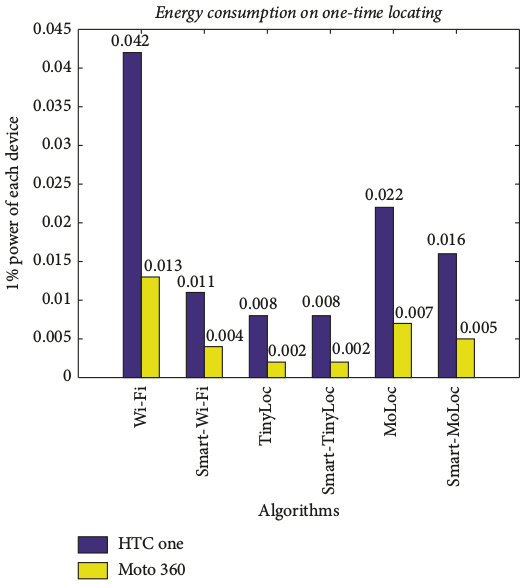
\includegraphics[width=0.6\textwidth]{img/smart_fix}
		\par\end{centering}
	\caption{Energy consumption based on prototypes (source: \cite{SmartFix})\label{fig:SmartFix}}
	\label{fig01c03}
\end{figure}

This paper proposed an tested new localization technology, SmartFix, which main focus is to improve energy efficiency on wearable devices. According to the experiment, probability of error within 2 meters can be reached in 80\% of cases. Meanwhile, energy consumption is 35\% lower than that of MoLoc with the same accuracy. Results show that implementing SmartFix obtains the best accuracy with minimal energy cost.

\section{Smartwatch vs. Smartphone}\label{sec:SWvsSP}
It is a comparative study about localization using smartwatch vs. smartphone \cite{SWvsSP} which presents that positioning accuracy using WiFi-based fingerprints implemented on smartwatch is sufficient for at least room-size locations. Average minimum room size is 10$m^2$ or at least 3$x$3 meters with maximum of five WiFi APs broadcasting using different channels.

Field study was conducted in six specific locations, such as farm, large room, house, two types of medium rooms and one small room. This study collected data using two Android-based devices, smartwatch MotoACTV was used and smartphone Samsung Galaxy S3 mini. To make fingerprint data more reliable the study also collects device orientation (horizontal, vertical) and data were taken in all four cardinal directions (north, east, south, west).

\begin{figure}[H]
	\begin{centering}
		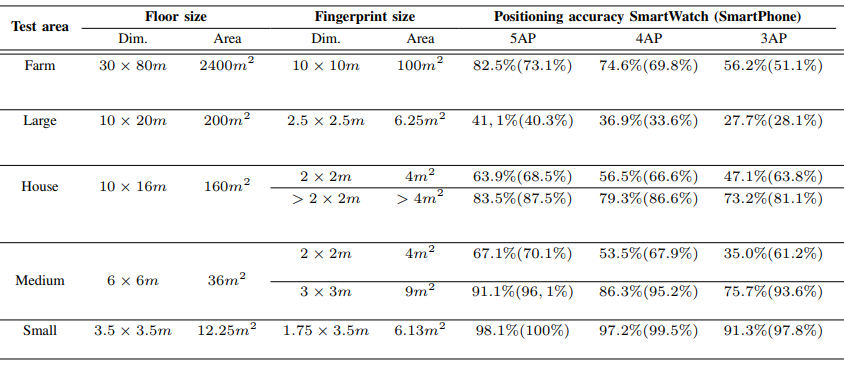
\includegraphics[width=0.9\textwidth]{img/smartwatch_vs_smartphone}
		\par\end{centering}
	\caption{Summary table of results (source: \cite{SWvsSP})\label{fig:SWvsSP}}
	\label{fig02c03}
\end{figure}

\fref{fig02c03} shows the results of these experiments. Most important part of this summary is comparison of positioning accuracy between smartwatch and smartphone. In all tests the difference in classification error between the smartphone and smartwatch was at most 5\% if all five APs were used. On the other hand it can be up to 25\% worse when using small amount of APs in large environments. This study confirms that localization using smartwatch can  be comparable to smartphone and sometimes even better for home environments. The usage of smartwatches is also preferable since it is tightly connected to a person.
